\documentclass{beamer}
\usepackage[size=a3,orientation=portrait,scale=1.65]{beamerposter}
\usetheme{LLT-poster}

\usepackage[utf8]{inputenc}
\usepackage[T1]{fontenc}
\usepackage{libertine}
\usepackage[scaled=0.92]{inconsolata}
\usepackage[libertine]{newtxmath}

\author{Justin Galminas, \: Emma Freeman, \: Kieran Jeffery, \: Oliver Barty}
\title{National Marine Aquarium Drawing Application}
\footimage{
\includegraphics[width=6cm]{images/plym-uni.png}}

\begin{document}
\begin{frame}[fragile]\centering

\begin{block}{Introduction}
    This is a COMP2003 project building an application for the National Marine Aquarium (NMA). The application allows aquarium attendees to draw their experiences, which are then scored by the aquarium to gain insight into what the Marine Park means to them.
    \vspace{1ex}

    The project is split into three major components - a frontend drawing application, an admin portal for managing data, and an API and database.
\end{block}

\begin{columns}[T]

\begin{column}{.46\textwidth}

    \begin{block}{Web and Android App Design}
        Users are able to submit drawings to the NMA using a web-based or Android drawing application. The web application was designed to be embedded into the NMA website, and the Android app was designed to run on low-powered tablets.
        \vspace{1ex}

        Both apps prioritise simplicity and intuitiveness, as they will often be used by young children. This means keeping the features simple - tools for pen, pencil, and brush, brush size, and a range of colours.
        \vspace{1ex}

        The web app is implemented with TypeScript and the React framework, and the Android app is written in Java using Android Studio.
        \vspace{1ex}

        \begin{center}
            
\includegraphics[width=0.75\linewidth]{images/web-app.png}
        \end{center}
    \end{block}

    \begin{block}{Admin Portal}
        The admin portal app allows the NMA staff to view records from the database and to add scores to drawings. It contacts the API to populate the UI with interactive tabular data.
        \vspace{1ex}

        It has one tab for each resource that can be managed - events, locations, and drawings. It also has a dashboard to display statistics and recently added drawings.
        \vspace{1ex}

        The portal is implemented using the same web technologies as the drawing app, but it uses Electron to compile as a native executable. 
        \vspace{1ex}

        \begin{center}
            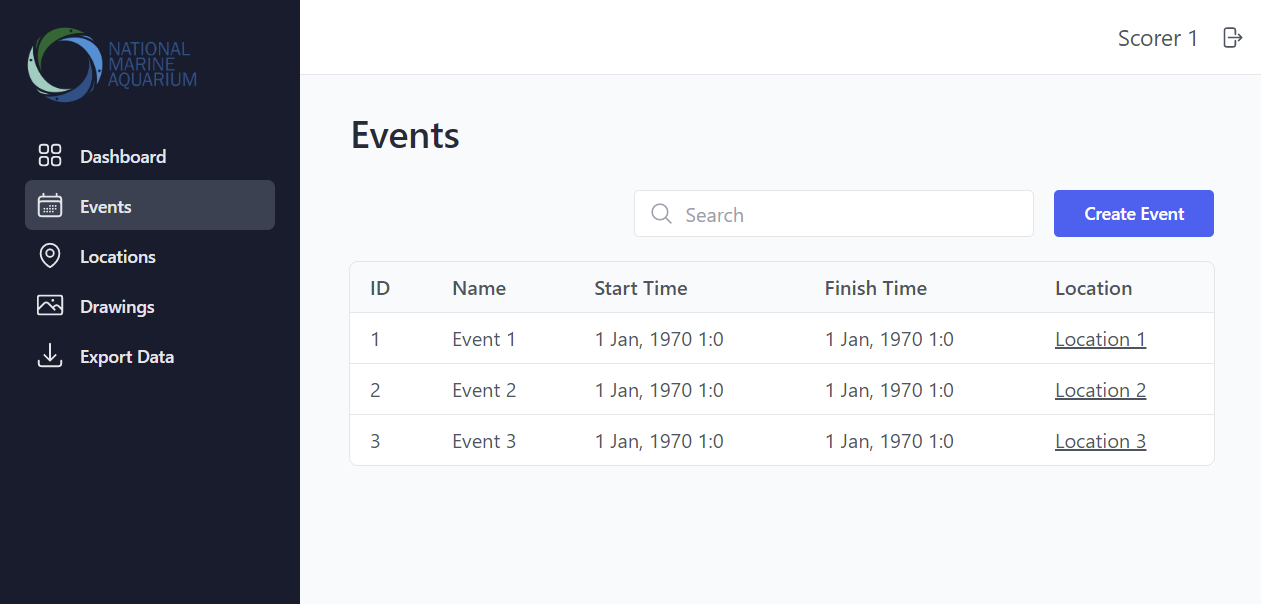
\includegraphics[width=0.75\linewidth]{images/admin-portal.png}
        \end{center}
    \end{block}

\end{column}

\begin{column}{.46\textwidth}

    \begin{block}{API}
        The API component allows programmatic access to the SQL database. It has endpoints for getting, creating, updating, and deleting records each SQL table, such as drawings and events. This is used by the drawing apps and the admin portal.
        \vspace{1ex}

        The API uses the Backblaze file hosting service API to store drawing images. This means the API can be hosted separately to the file storage, making hosting decoupled and much cheaper.
        \vspace{1ex}

        The API is implemented using C\#, with the EF Core ORM and ASP.NET web framework.
        \vspace{1ex}

        \begin{center}
            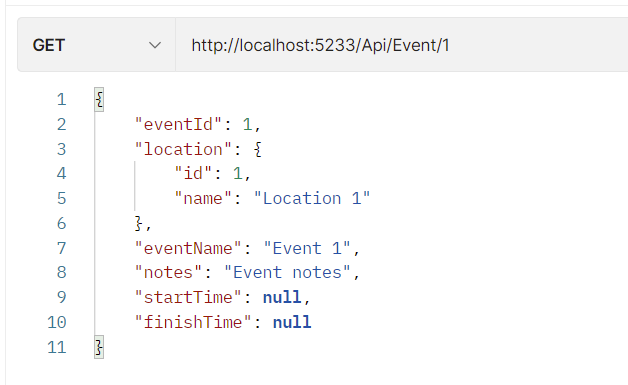
\includegraphics[width=0.6\linewidth]{images/api.png}
        \end{center}
    \end{block}

    \begin{block}{SQL Database}
        Data from the drawing app and admin portal is stored in a Microsoft SQL Server. This has several tables such as:
        \vspace{1ex}

        \begin{itemize}
            \item Drawing: an image filepath, the event it was made at, and its scores.
            \item Event: a name, location, and start/end times.
            \item Scorer: an NMA scorer username.
        \end{itemize}
        \vspace{1ex}

        \begin{center}
            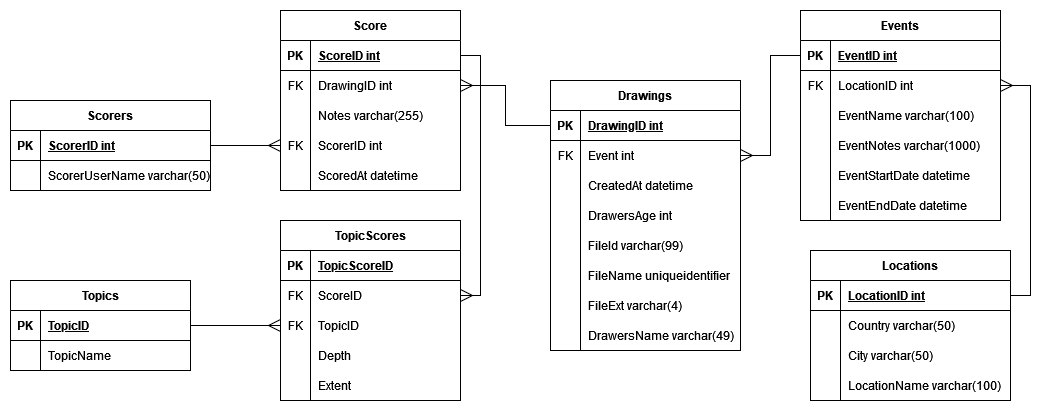
\includegraphics[width=0.65\linewidth]{images/erd.png}
        \end{center}
    \end{block}

    \begin{block}{Deployment}
        The web app, API, and SQL server can be built in Docker containers. This creates a reproducible build and runtime environment, which can then be deployed anywhere, such as to a cloud hosting server for the NMA to use.
        \vspace{1ex}

        The admin portal and Android app both build native executables for their respective platforms, which can then be directly run by the NMA and guests.
    \end{block}

\end{column}

\end{columns}

\end{frame}
\end{document}